%%%% ijcai16.tex

\typeout{IJCAI-16 Instructions for Authors}

% These are the instructions for authors for IJCAI-16.
% They are the same as the ones for IJCAI-11 with superficical wording
%   changes only.

\documentclass{article}
% The file ijcai16.sty is the style file for IJCAI-16 (same as ijcai07.sty).
\usepackage{ijcai16}

% Use the postscript times font!
\usepackage{times}

% the following package is optional:
%\usepackage{latexsym}

% Following comment is from ijcai97-submit.tex:
% The preparation of these files was supported by Schlumberger Palo Alto
% Research, AT\&T Bell Laboratories, and Morgan Kaufmann Publishers.
% Shirley Jowell, of Morgan Kaufmann Publishers, and Peter F.
% Patel-Schneider, of AT\&T Bell Laboratories collaborated on their
% preparation.

% These instructions can be modified and used in other conferences as long
% as credit to the authors and supporting agencies is retained, this notice
% is not changed, and further modification or reuse is not restricted.
% Neither Shirley Jowell nor Peter F. Patel-Schneider can be listed as
% contacts for providing assistance without their prior permission.

% To use for other conferences, change references to files and the
% conference appropriate and use other authors, contacts, publishers, and
% organizations.
% Also change the deadline and address for returning papers and the length and
% page charge instructions.
% Put where the files are available in the appropriate places.

%\usepackage{amsmath}

\usepackage{graphicx}

% use the algorithm packages
\usepackage{algorithm}               %format of the algorithm

\usepackage{algorithmic}             %format of the algorithm

\usepackage{multirow}                %multirow for format of table

%\usepackage{amsmath}

\usepackage{xcolor}


\begin{document}

%/DeclareMathOperator*{/argmin}{argmin}         %argmin或argmax公式的排版

%/renewcommand{/algorithmicrequire}{/textbf{Input:}}   %Use Input in the format of Algorithm

%/renewcommand{/algorithmicensure}{/textbf{Output:}}   %UseOutput in the format of Algorithm



\section{Explaining Why-not Questions}

\subsection{Problem Statement}

In this paper, we work with RDF graphs which is a collection of subject-property-object(SPO) triples.
Assume there are infinite sets $I$(IRIs), $B$(blank nodes) and $L$(RDF literals), then each triple $t$ formed
as $(s,p,o) \in (I \cup B) \times I \times (I \cup B \cup L)$ is either a pair of entities with a named relationship or an entity with named attribute and value.
For user queries, we mainly consider the basic select-project-join(SPJ) fragment of sparql queries
where the selection condition is a conjunction of triple patterns $P_1 \wedge \cdots \wedge P_l$.
Each $P_i$ is either a selection triple pattern “$(S_j$ $op$ $c)$” or a join triple pattern “$(S_j$ $op$ $S_k)$”,
where $S_i$ is a resource standing for either an entity or a class, $c$ is a literal, and $op$ is a predicate.

\textbf{\underline{Why-not Questions.}} Given an input sparql query $Q$ on a RDF graph $G$, let $Q(G)$ denote the result set of $Q$ on $G$. In the most basic form, a why-not question on $Q(G)$ is represented by a non-empty collection of why-not keywords $K=\{k_1,··· ,k_n \},n \geq 1$, where each why-not keyword $k_i$ can be mapped on $G$ with an entity $e_i$ and $e_i \notin Q(G)$. Corresponding to the why-not keywords, why-not instances is denoted as a non-empty set of instances $I=\{e_1, ··· , e_n\}$.

Essentially, the why-not question is asking why $I$ is not a subset of $Q(G)$; i.e., why each $e_i \in I$ is not in $Q(G)$. In the most general case, a user sparql query may contain multiple variables, thus a why-not question may be posed towards different variables which might cause ambiguity. By default, the select clause of sparql query limits the returned result and why-not questions are associated with the selected variables naturally. For simplicity and without loss of generality, we assume each why-not keyword responds to a specific variable within the user sparql query. Therefore, a why-not question on $Q(G)$ is represented by $WN=\{(k_1,v_1 ), \cdots ,(k_n,v_n)\},n \geq 1$ where each why-not pair $(k_i,v_i)$ is a why-not keyword $k_i$ and its related variable $v_i$. The default circumstance can be easily processed as the responding variable $v_i$ is set to $null$. In Example 1, the why-not question is represented by $WN=\{(┤),(┤)\}$.

\textbf{\underline{Query Pattern.}} Given a sparql query $Q$, the main component of $Q$ is the where clause which is a conjunction of triple patterns. Assume there is a set of variables $V$ disjoint from the sets $I$, $B$ and $L$, then each triple pattern is a triple $(v_1,v_2,v_3 ) \in (I \cup V) \times (I \cup V) \times (I \cup V \cup L)$. A query pattern is a set of triple patterns where the same variable in different patterns denotes a join condition. As a triple pattern can be viewed as a directed edge, a query pattern can be represented as a tree structure. In Example 1, the query pattern of user sparql query can be depicted as a tree in Fig2.

\textbf{\underline{Why-not Query.}} Given a sparql query $Q$, a why-not query $Q^*$ is a refined query which is derived from $Q$ with some modification operations. Since the modification operations may be various, we try to construct the why-not query with graph matching methods and preserve the most similar query pattern with $Q$. In essence, why-not query is a similar query pattern of $Q$ which can returns results containing the why-not instances.

\textbf{\underline{Explanation.}} Given a sparql query $Q$ and why-not questions $WN$,  the explanation for each why-not question is represented by $E=\{(tq_1, tw_1 ), \cdots, (tq_m, tw_m )\}, m \geq 1$, where $(tq_i, tw_i )$ is a RDF term pair, $tq_i$ is a RDF term in the user sparql query, $tw_i$ is a RDF term in the why-not query, and $tq_i \neq tw_i$. The explanation answers the why-not question by given a suggestion of modifying the RDF term $tq_i$ to a new RDF term $tw_i$.

Given the above statements, we formalize the problem of answering why-not questions to sparql queries on RDF databases as follows: Given an input sparql query $Q$, a RDF graph $G$, and why-not questions $WN$, the process of seeking why-not answers is to compute a reasonable explanation $E$. According to the explanation, users can either understand why her interested item is not in the result set or try to change the original query to gain the expected instances.

\subsection{Framework and Algorithms}

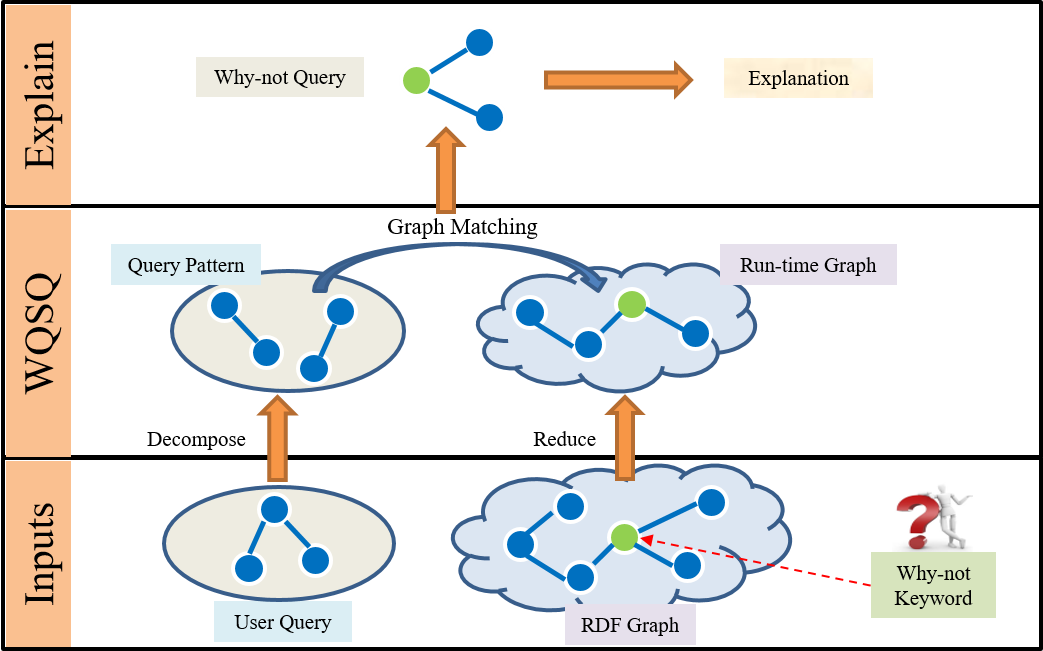
\includegraphics[width=3.36in]{framework.png}

\begin{center}
\textbf{Figure 3: Framework of WQSQ}
\end{center}

In this section, we propose a unified framework called $WQSQ$ (i.e., \textbf{W}hy-not \textbf{Q}uestions on \textbf{S}parql \textbf{Q}ueries) and present an overview of our approach to compute explanations for why-not questions by heuristically generating a refined why-not query. As illustrated in Figure 3, $WQSQ$ takes a sparql query, a RDF graph and why-not questions as input, and returns the refined sparql query with maximum similarity to users. Specifically, the explanation framework mainly consists of the following three steps:
(1)	Mapping why-not keyword on RDF graph.
(2)	Constructing why-not query.
(3)	Computing explanations.
Details of the framework will be discussed subsequently.

In the first step, we need to find the correct instance the user informed. The most simple way is to search the keyword on the RDF graph and returns the instance whose certain attribute value is the keyword. As the search method is executed as an exact matching process, this method always return empty or irrelevant results. For another aspect, if we use a similarity-based method to obtain all relevant instances whose value is similar with the keyword, then too many results would be returned. As a compromise, we use the latter approach to get some instances with a similarity threshold $\tau$ limited. After that, the syntax information of edges in query pattern is exploited to disambiguate the instance. Consequently, only a few instances are mapped from the why-not keyword, and we can utilize the similarity score of final constructed why-not graph to further differentiate them. What should be noticed is that, if no instances are mapped with the why-not keyword, then the framework finished at this step because it's meaningless to explain an absent instance in the RDF graph.

Secondly, the system adopts a graph pattern matching method to construct a why-not query, which is outlined in Algorithm 1. Before the matching, we decompose the query to several graph patterns(Line 1). The advantage of the pattern decomposing is that the whole matching procedure can be divided into series of iterations, where each iteration corresponds to a subgraph pattern matching. Hence the median result can be utilized to guide the matching direction. Several techniques concerning graph pattern decomposing has been proposed, such as edge based, star based, multi-way based, twin-twig based approach. In this paper, we adopt the edge based approach for simplicity and efficiency. The matching process is started from the why-not instance, so that we can guarantee the final constructed why-not query can return the user expected item. In the first iteration, we execute the match between all edges linked with why-not instance and all query patterns. For each matching process, we compute the similarity score between two edges. After the iteration, the edge and query pattern with the highest similarity score is preserved. Next for each iteration(lines 5-11), we find the matched edge to join into the graph generated in the former iteration(line 9). At last, a tree structure similar with user query rooted at the why-not instance is constructed. With the corresponding nodes been replaced with different variables(line 16), a why-not query is generated.

\begin{algorithm}[htb]         %算法的开始
\caption{ Construct a why-not query.} %算法的标题
\label{alg1:Framwork}                  %给算法一个标签,这样方便在文中对算法的引用
\begin{algorithmic}[1]                %这个1 表示每一行都显示数字

\REQUIRE ~~\\                         %算法的输入参数:Input
    Run-time Graph, $G_R$\\
    User Sparql Query, $Q$\\
    Why-not Instances of a certain keyword, $WI=\{wi_1,wi_2,\cdots,wi_m\}$

\ENSURE ~~\\                          %算法的输出:Output
    Ensemble of classifiers on the current batch,  $E_n$;

\STATE Decompose $Q$ into a collection of edges pattern $P=\{p_0, p_1, \cdots, p_l\}$;      %算法的一个陈述,对应算法的一个步骤或公式之类的; /label{ code:fram:extract }对此行的标记,方便在文中引用算法的某个步骤
\STATE Initial similar graph collection $G_s \leftarrow \emptyset $;
\FOR {each why-not instance $wi_j \in WI$}
\STATE $G_{wi_j}=(N_j, M_j);$  $N_j=\{wi_j\}$, $M_j=\emptyset;$  $score=0;$
\FOR {each pattern $p_i \in P $}
\FOR {each edge $e$ in linked edges of unmatched node $v$ in $N_j$}
\STATE $score += sim(e, p_i);$
\IF {$p_i.match(e)$}
\STATE $M_j.join(e);$  $N_j.add(e.neighbor(v));$
\ENDIF
\ENDFOR
\ENDFOR
\STATE $G_s.push(G_{wi_j});$
\ENDFOR
\STATE $sort(G_s);$  $Q_w=G_s.top1;$
\STATE replace the why-not instance in $Q_w$ with a variable $?x$;
\RETURN $Q_w$;                %算法的返回值

\end{algorithmic}
\end{algorithm}

%Lemma 1: The space complexity and time complexity of Algorithm 1 are O() and O() respectively.

%Proof Sketch:

After the why-not query is generated, we can return this refined query to the users as an answer to the why-not questions. However, the explanation is a little vague because of the coarsness. Thus we refined our work to compute a more clear and fine-grained explanation. The key idea is that we make a comparison to find the difference between constructed why-not query and user query. And each different place picked out as a term pair consists of the final explanation. The detailed process is illustrated in Algorithm 2.

\begin{algorithm}[htb]         %算法的开始
\caption{ Compute explanations.}      %算法的标题
\label{alg2:Framwork}                  %给算法一个标签,这样方便在文中对算法的引用
\begin{algorithmic}[1]                %这个1 表示每一行都显示数字

\REQUIRE ~~\\                         %算法的输入参数:Input
    User Sparql Query, $Q$\\
    Why-not Query, $Q_w$

\ENSURE ~~\\                          %算法的输出:Output
    Explanation Set of a why-not question,  $E$;

\FOR {each triple $t_w \in Q_w$}
\STATE find the matched triple $t$ in $Q$;
\STATE store the label pair $(t_w.s, t.s)$ $(t_w.p, t.p)$ $(t_w.o, t.o)$ in a map;
\ENDFOR
\FOR {each label pair $(l, r)$ in the map}
\IF {$l$ and $r$ are not variables \&\& $l \not = r$}
\STATE $E.add(pair(l, r))$
\ENDIF
\ENDFOR
\RETURN $E$;                %算法的返回值

\end{algorithmic}
\end{algorithm}

%Lemma 2: The space complexity and time complexity of Algorithm 2 are $O(M_Q)$ and $O(M_Q+2N_Q)$ respectively.

%Proof Sketch:




\subsection{Score Function}

In Algorithm 1, for each why-not instance, we construct a why-not query that can generate results containing the instance. Also we need the constructed query to be the most similar one to the user query. We use this idea as heuristic information and add it to the score function. For each iteration, the score of currently matched sub-graph is defined as follows:
$$ score(M_i) = score(M_{i-1}) + sim(t, p_i  ), (1-1)$$
where,
$$ sim(t, p) = sim(t_s, p_s ) + sim(t_p, p_p ) + sim(t_o, p_o ) ,$$
means the similarity between an edge $t$ and sub pattern $p_i$ .

\newtheorem{thm}{Theorem}[section]
\begin{thm}
Given the score function, the problem of construct a why-not query can be reduced to a dynamic programming problem.
\end{thm}

\textbf{Proof Sketch:} To prove this theorem, we need to verify whether the two key attributes as a dynamic programming problem must have in order applicable to this problem, which is optimal substructure and overlapping sub-problems, respectively. We will state that from two aspects:
(1) Optimal Substructure. Suppose the size of decomposed patterns is $t$, and after $i$ times matching, the constructed subgraph is $Gs_i$ with currently maximum score, $score(M_i)$. In next iteration, we explore the solution space to find an edge that is the most similar with query pattern $p_i$, which makes the second addend of formula (1-1) maximized, then $score(M_{i+1})$ is maximized, the matched edge is selected and joined to $Gs_i$ to generate $Gs_{i+1}$. Hence, the solution to a given optimization problem can be obtained by the combination of optimal solutions to its sub-problems.
(2) Overlapping Sub-problems. The process of constructing the why-not query can be decomposed a series of subroutines, we find a matched edge of a given query pattern and join into currently constructed subgraph. Suppose the final why-not graph is $Gs = e_1 \bowtie e_2 \bowtie \cdots \bowtie e_n$, then for the $i$th iteration, its sub-problems contains randomly joined $(i-1)$ edges. That is, for different iterations, the sub-problems may be overlapping.
Based on (1) and (2), the problem of constructing a why-not query satisfies the quality of optimal substructure and overlapping sub-problems, thus can be reduced to a dynamic programming problem, Theorem 3.1 holds.

From theorem 3.1, it is easy to deduce that with the well-defined score function, we can always find the most optimal solution in global. This guarantees that our algorithms can work in a correct and reasonable way.


\section{Optimization Strategies}

\subsection{Run-time Graph Construction}

Instead of loading the whole RDF graph $G$ into the main memory, we propose a method to load in a subgraph of $G$ without loss of useful information, which is called the run-time graph $G_R$ regarding $Q$. Considering the why-not question answering procedure, the necessary knowledge mainly covers the following two types of instance :

\begin{itemize}
\item Type-1 instance: which is mapped on the RDF graph by the why not keyword in the why-not question ,
\item Type-2 instance: which is covered by types in the user query.
\end{itemize}

Besides, the relation between the two types instance is also useful as we want to construct a query whose result covers the original instance and why-not instance as much as possible. Therefore, we extract the two kinds of instance at first, then add the linked path between type-1 instance and type-2 instance as auxiliary information. In a further step, for each type-2 instance, we only consider the linked edges labeled the same as the predicates in query pattern. Thus we use the edge information to remove useless relations and attributes of the type-2 instances. The detailed process is presented in Algorithm 3.


\begin{algorithm}[htb]         %算法的开始
\caption{ Construct a run-time graph.} %算法的标题
\label{alg3:Framwork}                  %给算法一个标签,这样方便在文中对算法的引用
\begin{algorithmic}[1]                %这个1 表示每一行都显示数字

\REQUIRE ~~\\                         %算法的输入参数:Input
    Global RDF Graph, $G$\\
    User Sparql Query, $Q$\\
    Why-not keywords, $K=\{k_1,k_2,\cdots,k_n\}$

\ENSURE ~~\\                          %算法的输出:Output
    Run-time Graph, $G_R$;

\STATE $QI \leftarrow \emptyset;$  $WI \leftarrow \emptyset;$  $G_R \leftarrow \emptyset;$;
\FOR {each variable $v_i$ of $Q$}
\STATE query instances $QI = \rho_G(v_i)$;
\ENDFOR
\STATE construct query instances graph $G_QI$ with $QI$;
\FOR {each keyword $k_i \in K $}
\STATE $G_{R_i} = (N_i, M_i)$;
\STATE why-not instances $WI_{k_i} = \rho_G(k_i)$;
\STATE disambiguate why-not instances with edges in $Q$;
\FOR {each instance $t \in QI$}
\STATE $N_i.add(t);$  $M_i.add(linked edges of t);$
\STATE compute joint path $p$ between $t$ and remain instances;
\STATE $N_i.add(p.nodes);$  $M_i.add(p.edges);$
\STATE add nodes and edges of $G_QI$ into $G_{R_i}$;
\ENDFOR
\STATE $G_R.push(G_{R_i})$;
\ENDFOR
\RETURN $G_R$;                %算法的返回值

\end{algorithmic}
\end{algorithm}

%Lemma 3: The space complexity and time complexity of Algorithm 3 are O() and O() respectively.

%Proof Sketch:


\subsection{Order-aware Graph Pattern Matching}
\textbf{Definition:} (Operator $\prec$) For any two decomposed edge patterns $p_i$  and $p_j$ in $Q$, $p_i \prec p_j$ if and only if one of the three conditions holds:
\begin{itemize}
\item $d(p_i) < d(p_j)$ ,
\item $d(p_i) = d(p_j)$ and $|\sigma_G (p_i)| < |\sigma_G (p_j)|$ ,
\item $d(p_i) = d(p_j)$ and $|\sigma_G (p_i )| = |\sigma_G (p_j)|$ and $id(p_i ) < id(p_j )$ .
\end{itemize}

where $d(p_i)$ is the depth of $p_i$ in the query tree, $|\sigma_G(p_i)|$ is the frequency of occurrences of pattern $p_i$ in the RDF graph, and $id(p_i)$ is the unique identifier of pattern $p_i$ assigned with an integer.

\begin{thm}

Given a pattern decomposition $\mathcal{D}^{'} = \{p_0^{'}, p_1^{'}, \cdots, p_t^{'}\}$ of $Q$ where each  $p_i^{'}(0 \leq i \leq t)$ is an edge, let $\mathcal{D} = \{p_0, p_1, \cdots, p_t\}$ be the decomposition constructed with order-aware strategy, then $\mathcal{D}$ is better than $\mathcal{D}^{'}$ to find the best match of $Q$.

\end{thm}


%\begin{Proof}

\textbf{Proof Sketch:}

Intuitively, as the query can be regarded as a tree, it is helpful to match the pattern with shallow and exact information earlier. For the first aspect, the why-not instance is more likely to be the root node or in a top layer, therefore, choose the edge pattern with lower depth in prior is better than the edge pattern with deeper depth. This can be depicted by the first condition. For another part, if two patterns have the same depth, then the pattern with lower frequency of occurrence is better because of the lower space to be selected. And this can be described by the second condition. At last, if the depth and frequency are accidently the same of the two patterns, then it’s not important to choose which pattern to be matched, thus we just use the pattern id to differentiate the patterns, which is reflected by the third condition. By the above analysis, it is apparently the order-aware pattern matching is better than no orders as the former reduce the unrelated matches in each iteration as much as possible.
%\end{Proof}

\end{document}
